% !TeX program = xelatex 

\PassOptionsToPackage{prologue, dvipsnames}{xcolor}
\documentclass[AutoFakeBold,AutoFakeSlant]{beamer}
\usetheme{metropolis}           % Use metropolis theme
\setbeamercovered{transparent}
\usepackage{listings}
\usepackage{grid-system}
\usepackage{ThinctPPT}
\usepackage[font=normalsize,labelfont=sf,textfont=sf]{subcaption} % Use only subcaption, not subfig
 
% 支持中文的设置
\usepackage{xeCJK}
\usepackage{fontspec}
\setCJKmainfont[ItalicFont=思源宋体,BoldFont=SourceHanSerifSC-Bold]{Source Han Serif SC}
\newcommand{\KaiTi}{\CJKfontspec{楷体}}%用命令\fzkaiti调用方正楷体简体

% other packages
\usepackage{latexsym,amsmath,xcolor,multicol,booktabs,calligra}
\usepackage{graphicx,pstricks,listings,stackengine}
\usepackage{wrapfig}
\usepackage[english]{babel}
\usepackage[font=normalsize,labelfont=sf,textfont=sf]{subcaption}

\title{\textbf{2023}\\年终总结}
\date{\today}
\author{
\includegraphics[width=0.26\linewidth]{logo}\\软件部~/~王升平}
\begin{document}
	\maketitle
	
	\section{过去一年的数据}
	\subsection{BUG数据}
	
	\begin{frame}[fragile]
		\LogoFrametitle{2023年度发现的BUG统计图表}
		\begin{figure}
			\centering % 将整个 figure* 居中
			\begin{subfigure}{\linewidth}
				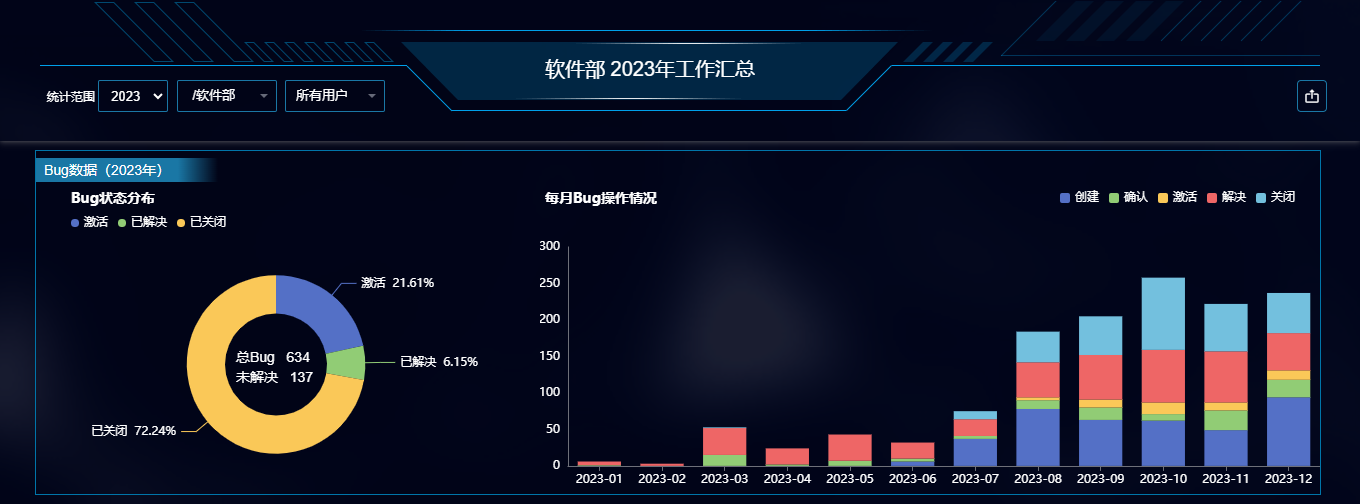
\includegraphics[width=\linewidth]{bug}
			\end{subfigure}
		\end{figure} 
		
		\begin{minipage}[l]{0.3\linewidth}
			\large
			总BUG数 : 634 \\
			未解决  : 137
		\end{minipage}\hfill
		\begin{minipage}[l]{0.6\linewidth}
			\footnotesize
			上半年主要程序刚发布,只做了一些简单的交互测试,发现的BUG较少.下半年产品用户越来越多,产品和用户以及自身的测试团队组建一同发现BUG,导致BUG激增。
		\end{minipage}
	\end{frame}
	
	
	\subsection{测试用例数据}
	\begin{frame}[fragile]
		\LogoFrametitle{2023年度测试用例统计图表}
		\begin{figure}
			\centering % 将整个 figure* 居中
			\begin{subfigure}{\linewidth}
				\includegraphics[width=\linewidth]{Task}
			\end{subfigure}
			
			\begin{minipage}[l]{0.3\linewidth}
				\large
				总BUG数 : 634 \\
				未解决  : 137
			\end{minipage}\hfill
			\begin{minipage}[l]{0.6\linewidth}
			\footnotesize
			上半年之前只有一个测试人员.并且兼做开发任务。下半年开始随着测试团队扩大,用户反馈增多,测试用例也越来越细化。
			\end{minipage}
		\end{figure} 
	\end{frame}
	

	
	\subsection{开发任务数据}
	\begin{frame}[fragile]
		\LogoFrametitle{2023年度开发任务统计图表}
		\begin{figure}
			\centering % 将整个 figure* 居中
			\begin{subfigure}{\linewidth}
				\includegraphics[width=\linewidth]{Task}
			\end{subfigure} 
			
			\begin{minipage}[l]{0.3\linewidth}
				\large
				总任务数 : 204 \\
				未完成  : 20
			\end{minipage}\hfill
			\begin{minipage}[l]{0.6\linewidth}
				\footnotesize
				上半年主要是程序的维护和准备发布阶段,任务主要在发布前后有激增.下半年主要随着团队人员增加,自九月份开始任务量逐渐形成递增态势.
			\end{minipage}
		\end{figure}
	\end{frame}
	
	
\end{document}
